\documentclass[wide,a4paper,titlepage,12pt] {article}
\usepackage{polski}
\usepackage[UTF8]{inputenc}
\usepackage{listings}
\usepackage{slashbox}
\usepackage[table]{xcolor}
\usepackage{graphicx,pdflscape}
\usepackage{placeins}
\usepackage{reportshelper}

\title{Schemat Aproksymacyjny dla $P_{2}||C_{max}$}
\author{Jacek Wieczorek (181043)}

% Title page layout (fold)
\makeatletter
\renewcommand{\maketitle}{
  \begin{titlepage}
    \begin{center}
      \vspace*{3cm}
      \LARGE \@title \par
      \vspace{2cm}
      \textit{\small Autorzy:}\par
      \normalsize \@author\par \normalsize
      \vspace{3cm}
      Prowadzący : mgr inż. Karolina Mokrzysz\\
      Poniedziałek TP 11.00 - 13.00\\
      \vspace{3cm}
      Wydział Elektroniki\\ III rok \par
      \vspace{3cm}
      \small \@date
    \end{center}
  \end{titlepage}
}
\makeatother

\begin{document}
  \maketitle
  \section{Opis problemu}
\paragraph{}
 Celem laboratorium jest zaimplementowanie algorytmu szeregowania $n$ zadań na $2$ równolegle działających procesorach -  $P_{2} || C_{max}$ za pomocą wilomianowego schematu aproksymacyjnego \textit{PTAS}.

\section{PTAS}
\paragraph{}
Wielomianowy schemat aproksymacji (ang. Polynomial-time approximation scheme, w skrócie PTAS) to algorytm aproksymacyjny, który pozwala na uzyskanie dowolnie dobrego rozwiązania przybliżonego danego problemu optymalizacyjnego, i którego złożoność czasowa jest wielomianowa dla każdej żądanej dokładności.

\paragraph{}
Algorytm $A$ jest wielomianowym schematem aproksymacji dla problemu $\Pi$ jeśli spełnione są następujące warunki:
\begin{itemize}
    \item dla każdego odpowiedniego $\varepsilon$ A jest algorytmem $\varepsilon$-aproksymacyjnym dla $\Pi$,
    \item dla każdego odpowiedniego $\varepsilon$ złożoność czasowa $A$ jest wielomianowa ze względu na rozmiar instancji problemu podanej na wejściu $A$.
\end{itemize}

\section{Opis algorytmu}
\paragraph{}
\begin{itemize}
  \item Krok 1 : Posortuj zadania malejąco wg czasu ich wykonania
  \item Krok 2 : Przyporządkuj $k$-pierwszych zadań w sposób optymalny
  \item Krok 3 : Pozostałe $n-k$ zadań przyporządkuj za pomocą algorytmu \textit{LPT} 
\end{itemize}

\section{Dowód wielomianowości}
\paragraph{}
\begin{itemize}
  \item Sortowanie: $O(nlogn)$
  \item Przyporządkowanie 1 : przegląd zupełny przy pomocą wektora binarnego - $2^k$
  \item Przyporządkowanie \textit{LPT} : $O(n-k)$
\end{itemize}

\paragraph{}
Złożóność obliczeniowa : $O(nlogn + 2^k)$
\paragraph{}
Dokładność : 
$\varepsilon = \frac{1}{1+\lfloor k/2 \rfloor}$
\paragraph{}
 Wynika z tego, iż k = $O(\frac{1}{\varepsilon})$
\paragraph{}
Co daje nam złożoność obliczeniową algorytmu : $O(nlogn + 2^{\frac{1}{\varepsilon}})$

\section{Implementacja}
\paragraph{}
\putcode{code/algo.cs}{java}

\section{Testy}
\paragraph{}
W celu przeprowadzenia dokłądnej analizy wykonanych zostało szereg testów badających czas wykonania algorytmu w zależności od parametru $n$ i $\varepsilon$. W przypadku badania zcasu wykonania kazdej instancji wykonano po 3 testy, a prezentowany wynik jest ich średnią arytmetyczną. Mimo iż program posiada graficzny interfejs użytkownika, moduł testowy wykonany został jako aplikacja konsolowa.

\end{document}



% \begin{figure}[htbp]
 %     \begin{center}
  %      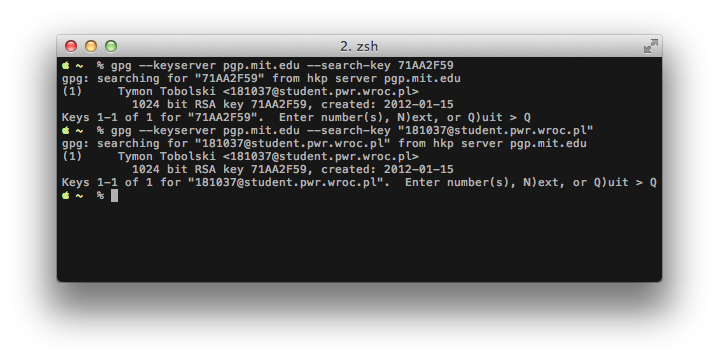
\includegraphics[scale=0.5]{screen/11.png}
   %     \caption{}
    %  \end{center}
    %\end{figure}